\documentclass[12pt,a4paper,openright,twoside]{book}
\usepackage[utf8]{inputenc}
\usepackage{algorithm}
\usepackage{algpseudocode}
\usepackage{amsmath}
\usepackage{amsthm}
\usepackage{amssymb}
\usepackage{bm}
\usepackage{colortbl}
\usepackage{graphicx}
\usepackage{geometry}
\usepackage{hyperref}
\usepackage{ifthen}
\usepackage{latexsym}
\usepackage{listings}
\usepackage{makeidx}
\usepackage{minted}
\usepackage{tikz}
\usepackage{titlesec}
\usepackage{wrapfig}
\usepackage{xcolor}
\definecolor{mygreen}{rgb}{0,0.6,0}
\definecolor{mygray}{rgb}{0.5,0.5,0.5}
\definecolor{mymauve}{rgb}{0.58,0,0.82}
\definecolor{mygreen}{rgb}{0,0.6,0}
\definecolor{mygray}{rgb}{0.5,0.5,0.5}
\definecolor{mymauve}{rgb}{0.58,0,0.82}

\lstset{
  basicstyle=\ttfamily,
  language=Python,
  commentstyle=\color{mygreen},
  keywordstyle=\color{blue},
  numberstyle=\tiny\color{mygray},
  stringstyle=\color{mymauve},
  numbers=left,
  showstringspaces=false,
  extendedchars=true,
  breaklines=true,              % A capo automatico per righe lunghe
  breakatwhitespace=false,     % Non limitare l'a capo agli spazi
  breakautoindent=true,        % Mantieni indentazione dopo l'a capo
  postbreak=\mbox{\textcolor{red}{$\hookrightarrow$}\space} % Indicatore visivo dell'a capo
}
\graphicspath{ {./img/} }

\newcommand{\qvec}[1]{	extbf{	extit{#1}}}
\newcommand{\mathbi}[1]{	extbf{\em #1}}
\newcommand{\TODOComment}[1]{}
\newcommand{\underlinebrace}[2]{%
\tikz[remember picture,baseline=(a.base)]{%
\node[inner sep=0pt] (a) {#1}; 
\draw[decorate,decoration={brace,mirror,amplitude=4pt}] (a.south west) -- (a.south east);
\node[below=4pt] at (a.south) {#2};
}%
}
\begin{document}
\title{Post-Quantum Cryptography}
\author{Matteo Vanni}
\date{\today}
 
\newgeometry{margin=0.8in}
\begin{titlepage}
\begin{center}
 
    \large
    \textbf{ALMA MATER STUDIORUM -- UNIVERSITÀ DI BOLOGNA\\CAMPUS DI CESENA}
\\
    \noindent\hrulefill
    \vspace{0.4cm}
 
    \Large
    Corso di Laurea triennale in Ingegneria e Scienze Informatiche\\
 
    \Huge
    \vspace{4.5cm}
    \Large
    \textbf{
        Image Denoising Technique with Neural Network
   }
 
    \large
    \vspace{1cm}
 
    \vspace{5.5cm}
    \begin{minipage}[t]{0.64\textwidth}
      \begin{flushleft}
        \textit{Relatore:}\\
        \textbf{Prof. Lazzaro Damiana}
        \\
        \vspace{0.4cm}
        \textit{Co/Contro Relatore}\\
        \textbf{Dott. Ezio Greggio}
      \end{flushleft}
    \end{minipage}
    \begin{minipage}[t]{0.34\textwidth}
      
      \begin{flushright}
        \textit{Candidato:}\\
        \textbf{Matteo Vanni}
\\
        \textit{Matricola: 0000935584}
      \end{flushright}

    \end{minipage}\\
 
    \vfill
    \noindent\hrulefill

    \textit{MMMCAINA 20256}
    \vspace{0.3cm}
    \Large
 
  \end{center}
\end{titlepage}
 
\titleformat{\chapter}{\normalfont\huge \bfseries}{\Huge \thechapter}{20pt}{\Huge}
\tableofcontents

\chapter{Articolanzio}
\section{Panoramica sul problema}
L'image denoising è il processo di rimozione di rumore da un'immagine.\\
Il rumore, che è causato da svariate fonti, quali foto fatte in condizioni di scarsa illuminazione o problemi che corrompono i file, causa perdita d'informazione sull'immagine.
\paragraph{Cos è il rumore?} 
Un aggiunta casuale di pixel che non appartengono all'immagine originale e ce ne sono di varie tipologie:\\
Impulse Noise(IN) dove i pixel sono completamente diversi da quelli attorno. Esistono due categorie di IN: Salt and Pepper Noise(SPN) e Random Valued Impulse Noise(RVIN).\\
Additive White Gaussian Noise(AWGN) cambia ogni pixel dall'originale di una piccola quantità.\\

\section{Utilizzo di modelli di Deep Learning}
\'E essenziale rimuovere il rumore e ristabilire l'immagine originale dove 
riottenere l'immagine originale è importante per prestazioni robuste o ricostruire le informazioni mancanti è molto utile, come immagini astronomiche di oggetti molto lontani.\\
Le reti neurali convoluzionali lavorano bene con le immagini e ne utilizzeremo N, menzionate in alcuni paper di ricerca e compareremo i risultati di ogni modello.\\

\section{Dataset utilizzati}
Il primo dataset usato per addrestrare i modelli sarà Oxford-IIIT Pet da Tensorflow, in modo poi da testare i modelli con immagini che non conoscono da altri dataset(colonscopie)\\
\begin{lstlisting}{python}
def load_dataset(split='train', img_size=(256,256), batch_size=16):
    #Carica il dataset Oxford-IIIT Pet da tfds e applica il #preprocessamento.

    #Ritorna un dataset in batch.

    # as_supervised=False per mantenere dict
    dataset = tfds.load('oxford_iiit_pet', split=split, as_supervised=False) 
    # Preprocessing
    dataset = dataset.map(lambda sample: preprocess(sample, img_size))  
    # Ottimizza il caricamento
    dataset = dataset.shuffle(1024).batch(batch_size).prefetch(tf.data.AUTOTUNE)  
    return dataset
\end{lstlisting}\\

\begin{minted}{python}
  import numpy as np
      
  def incmatrix(genl1,genl2):
      m = len(genl1)
      n = len(genl2)
      M = None #to become the incidence matrix
      VT = np.zeros((n*m,1), int)  #dummy variable
      
      #compute the bitwise xor matrix
      M1 = bitxormatrix(genl1)
      M2 = np.triu(bitxormatrix(genl2),1) 
  
      for i in range(m-1):
          for j in range(i+1, m):
              [r,c] = np.where(M2 == M1[i,j])
              for k in range(len(r)):
                  VT[(i)*n + r[k]] = 1;
                  VT[(i)*n + c[k]] = 1;
                  VT[(j)*n + r[k]] = 1;
                  VT[(j)*n + c[k]] = 1;
                  
                  if M is None:
                      M = np.copy(VT)
                  else:
                      M = np.concatenate((M, VT), 1)
                  
                  VT = np.zeros((n*m,1), int)
      
      return M
\end{minted}

Kvasir-seg: 1000(MILLEH) immagini di polipi, 

gli animali di arvard, le colonscopie \TODOComment{Approfondire aggiungendo link ai dataset e approfondire cose che non ci sono}

\chapter{Decsrizione delle reti}
\section{Rumore}
La prima funzione di rumore è u'aggiunta di rumore casuale a ogni pixel dell'immagine.\\
\begin{lstlisting}{python}
  def add_noise(x, noise_factor=0.1):
    """
    x: immagine in input
    noise_factor: fattore di rumore da aggiungere
    Ritorna:
      x_noisy: immagine con rumore aggiunto
    """
    noise = tf.random.normal(shape=tf.shape(x), mean=0.0, stddev=1.0)
    x_noisy = x + noise_factor * noise
    return x_noisy
\end{lstlisting}
E FAI RUMORE \textbf{QUIIIIIIIIIIIIIIIIIIIIIIIIIIIII}
Prima funzione di rumore -> Random noise con fattore 0.3 massimo
\TODOComment{questi 2 più avanti}
Rumore gaussiano 
Rumore a più layer


\section{Autoencoder}
Il primo approccio è stato quello di usare l'autencoder dell'articolo da cui sto copiando paro paro tutto.\\
Spiegazione del numero di layer usati e del tipo di mse loss fun, dam e learning rate di 1e-3
\begin{lstlisting}{python}
def build_autoencoder(input_shape):
    """
    Costruisce un autoencoder convoluzionale per immagini a colori.
    Parametri:
      input_shape: forma dell'immagine in input (es. (32,32,3))
    Ritorna:
      autoencoder: modello compilato
    """
    input_img = Input(shape=input_shape)

    # Encoder
    x = Conv2D(64, (3,3), activation='relu', padding='same')(input_img)
    x = MaxPooling2D((2,2), padding='same')(x)
    x = Conv2D(64, (3,3), activation='relu', padding='same')(x)
    encoded = MaxPooling2D((2,2), padding='same')(x)

    # Decoder
    x = Conv2D(64, (3,3), activation='relu', padding='same')(encoded)
    x = UpSampling2D((2,2))(x)
    x = Conv2D(64, (3,3), activation='relu', padding='same')(x)
    x = UpSampling2D((2,2))(x)
    decoded = Conv2D(3, (3,3), activation='sigmoid', padding='same')(x)

    autoencoder = Model(input_img, decoded)
    autoencoder.compile(optimizer='adam', loss='binary_crossentropy', metrics=['accuracy'])

    return autoencoder

autoencoder = build_autoencoder(input_shape=(img_size[0], img_size[1], 3))
autoencoder.summary()
\end{lstlisting}

\TODOComment{Modificare il dataset per i cosi successivi}

\section{RIDNet}
stessa cosa dell'autencoder (vedere se aggiungere tutto il codice gigante del setup)
\begin{lstlisting}{python}
  # MeanShift: sottrae (o aggiunge) la media RGB
@register_keras_serializable("MeanShift")
class MeanShift(Layer):
    def __init__(self, rgb_mean, sign=-1, **kwargs):
        """
        rgb_mean: tupla con la media dei canali R, G, B.
        sign: -1 per sottrarre la media, 1 per aggiungerla.
        """
        super(MeanShift, self).__init__(**kwargs)
        self.rgb_mean = tf.constant(rgb_mean, dtype=tf.float32)
        self.sign = sign

    def call(self, x):
        # x è atteso in formato (batch, altezza, larghezza, 3)
        # Sfruttiamo Lambda per eseguire l'operazione per ogni elemento
        # Nota: non stiamo scalando per std in questo esempio
        return x + self.sign * self.rgb_mean

# BasicBlock: Conv2D seguita da attivazione ReLU
@register_keras_serializable("BasicBlock")
class BasicBlock(Layer):
    def __init__(self, out_channels, kernel_size=3, stride=1, use_bias=False, **kwargs):
        super(BasicBlock, self).__init__(**kwargs)
        self.conv = Conv2D(out_channels, kernel_size, strides=stride,
                           padding='same', use_bias=use_bias)
        self.relu = ReLU()

    def call(self, x):
        return self.relu(self.conv(x))

# ResidualBlock: due convoluzioni con skip connection(come lavora cuda con 2 thread -> 2 filtri applicati e poi si uniscono i risultati)
@register_keras_serializable("ResidualBlock")
class ResidualBlock(Layer):
    def __init__(self, out_channels, **kwargs):
        super(ResidualBlock, self).__init__(**kwargs)
        self.conv1 = Conv2D(out_channels, 3, strides=1, padding='same')
        self.relu = ReLU()
        self.conv2 = Conv2D(out_channels, 3, strides=1, padding='same')

    def call(self, x):
        residual = self.conv1(x)
        residual = self.relu(residual)
        residual = self.conv2(residual)
        out = Add()([x, residual])
        return ReLU()(out)

# EResidualBlock: versione estesa con convoluzioni a gruppi
@register_keras_serializable("EResidualBlock")
class EResidualBlock(Layer):
    def __init__(self, out_channels, groups=1, **kwargs):
        super(EResidualBlock, self).__init__(**kwargs)
        self.conv1 = Conv2D(out_channels, 3, strides=1, padding='same', groups=groups)
        self.relu = ReLU()
        self.conv2 = Conv2D(out_channels, 3, strides=1, padding='same', groups=groups)
        self.conv3 = Conv2D(out_channels, 1, strides=1, padding='valid')

    def call(self, x):
        residual = self.conv1(x)
        residual = self.relu(residual)
        residual = self.conv2(residual)
        residual = self.relu(residual)
        residual = self.conv3(residual)
        out = Add()([x, residual])
        return ReLU()(out)

# Merge_Run_dual: due rami convoluzionali con dilatazioni diverse, poi fusione e skip connection
@register_keras_serializable("MergeRunDual")
class MergeRunDual(Layer):
    def __init__(self, out_channels, **kwargs):
        super(MergeRunDual, self).__init__(**kwargs)
        # Primo ramo
        self.conv1a = Conv2D(out_channels, 3, strides=1, padding='same')
        self.relu1a = ReLU()
        self.conv1b = Conv2D(out_channels, 3, strides=1, padding='same', dilation_rate=2)
        self.relu1b = ReLU()
        # Secondo ramo
        self.conv2a = Conv2D(out_channels, 3, strides=1, padding='same', dilation_rate=3)
        self.relu2a = ReLU()
        self.conv2b = Conv2D(out_channels, 3, strides=1, padding='same', dilation_rate=4)
        self.relu2b = ReLU()
        # Gogeta
        self.conv3 = Conv2D(out_channels, 3, strides=1, padding='same')
        self.relu3 = ReLU()

    def call(self, x):
        branch1 = self.relu1a(self.conv1a(x))
        branch1 = self.relu1b(self.conv1b(branch1))

        branch2 = self.relu2a(self.conv2a(x))
        branch2 = self.relu2b(self.conv2b(branch2))

        merged = Concatenate()([branch1, branch2])
        merged = self.relu3(self.conv3(merged))
        return Add()([merged, x])

# CALayer: Channel Attention Layer
@register_keras_serializable("CALayer")
class CALayer(Layer):
    def __init__(self, channel, reduction=16, **kwargs):
        super(CALayer, self).__init__(**kwargs)
        self.channel = channel
        self.reduction = reduction
        self.conv1 = Conv2D(channel // reduction, 1, strides=1, padding='same')
        self.relu = ReLU()
        self.conv2 = Conv2D(channel, 1, strides=1, padding='same', activation='sigmoid') #sigmoid: risultato tra 0 e 1

    def call(self, x):
        # Calcolo della media globale per canale
        y = tf.reduce_mean(x, axis=[1, 2], keepdims=True)
        y = self.relu(self.conv1(y))
        y = self.conv2(y)
        return Multiply()([x, y])

# Block: combinazione di MergeRunDual, ResidualBlock, EResidualBlock e CALayer
@register_keras_serializable("Block")
class Block(Layer):
    def __init__(self, out_channels, **kwargs):
        super(Block, self).__init__(**kwargs)
        self.merge_run_dual = MergeRunDual(out_channels)
        self.residual_block = ResidualBlock(out_channels)
        self.e_residual_block = EResidualBlock(out_channels)
        self.ca = CALayer(out_channels)

    def call(self, x):
        r1 = self.merge_run_dual(x)
        r2 = self.residual_block(r1)
        r3 = self.e_residual_block(r2)
        out = self.ca(r3)
        return out

# RIDNET: il modello final
@register_keras_serializable("RIDNET")
def RIDNET(n_feats=64, rgb_range=1.0):
    """
    n_feats: numero di feature channels usate all'interno del modello.<br>
    rgb_range: scala dei valori RGB (ad es. 1.0 se l'input è normalizzato [0,1]).
    """
    rgb_mean = (0.4488, 0.4371, 0.4040)

    input_layer = Input(shape=(None, None, 3))

    # Sottosottrai la media (MeanShift con sign=-1)
    sub_mean = MeanShift(rgb_mean, sign=-1)
    x = sub_mean(input_layer)

    # Testa: BasicBlock (conv + ReLU)
    head = Conv2D(n_feats, 3, strides=1, padding='same', activation='relu')(x)

    # Serie di blocchi
    b1 = Block(n_feats)(head)
    b2 = Block(n_feats)(b1)
    b3 = Block(n_feats)(b2)
    b4 = Block(n_feats)(b3)

    # Coda: convoluzione finale per ottenere 3 canali
    tail = Conv2D(3, 3, strides=1, padding='same')(b4)

    # Aggiungi la media (MeanShift con sign=+1)
    add_mean = MeanShift(rgb_mean, sign=1)
    res = add_mean(tail)

    # Connessione residua a livello di immagine: somma con l'input originale
    output = Add()([res, input_layer])

    model = Model(inputs=input_layer, outputs=output)
    return model

model = RIDNET(n_feats=32, rgb_range=1.0)
model.compile(optimizer='adam', loss='mse', metrics=['accuracy'] )
model.summary()

\end{lstlisting}

\chapter{Analisi ed ottimizzazione}
\section{Prestazioni}
PSNR è il metodo più comune per misurare la qualità delle immagini.\\
Il PSNR è definito come il rapporto tra il massimo valore possibile di un segnale e il valore del rumore che disturba la qualità della sua rappresentazione.\\ Normalmente misurato in una scala logaritmica in decibel(dB).\\
Data l'immagine originale(\textit{g}) e l'immagine rumorosa(\textit{f}), il PSNR è definito come: \[PSNR=20log_{10}(\frac{MAX_f}{\sqrt{MSE}})\] dove $MAX_f$ è il valore massimo del pixel dell'immagine e si calcola come \[MSE=\frac{1}{mn}\sum_{0}^{m-1}\sum_{0}^{n-1}||f(i,j)-g(i,j)||^2  \] mentre $MSE$(\textit{Mean Square Error}) è l'errore quadratico medio tra l'immagine originale e quella rumorosa.\\
\section{Prima run}
Il primo allenamento è stato sottoposto a entrambi i modelli con immagini RGB con risoluzione 112x112 pixel, un noise\_factor di 0.4 e 50 epoche di training.\\
Per l'autoenconcoder è stata usata una batch\_size di 16 mentre per la RIDNet una di 20.\\
\subsection{Autoencoder}
Model: "functional"\\
\begin{tabular}{|| c | c | c ||}
  \hline
  Layer (type) & Output Shape & Param \# \\
  \hline
  input\_layer & (None, 112, 112, 3) & 0 \\
  \hline
  conv2d & (None, 112, 112, 64) & 1,792 \\
  \hline
  max\_pooling2d & (None, 56, 56, 64) & 0 \\
  \hline
  conv2d\_1 & (None, 56, 56, 64) & 36,928 \\
  \hline
  max\_pooling2d\_1 & (None, 28, 28, 64) & 0 \\
  \hline
  conv2d\_2 & (None, 28, 28, 64) & 36,928 \\
  \hline
  up\_sampling2d & (N one, 56, 56, 64) & 0 \\
  \hline
  conv2d\_3 & (None, 56, 56, 64) & 36,928 \\
  \hline
  up\_sampling2d\_1 & (None, 112, 112, 64) & 0 \\
  \hline
  conv2d\_4 & (None, 112, 112, 3) & 1,731 \\
  \hline  
\end{tabular}

 Total params: 114,307 (446.51 KB)\\
 Trainable params: 114,307 (446.51 KB)\\
 Non-trainable params: 0 (0.00 B)\\
\begin{figure}
  \centering
  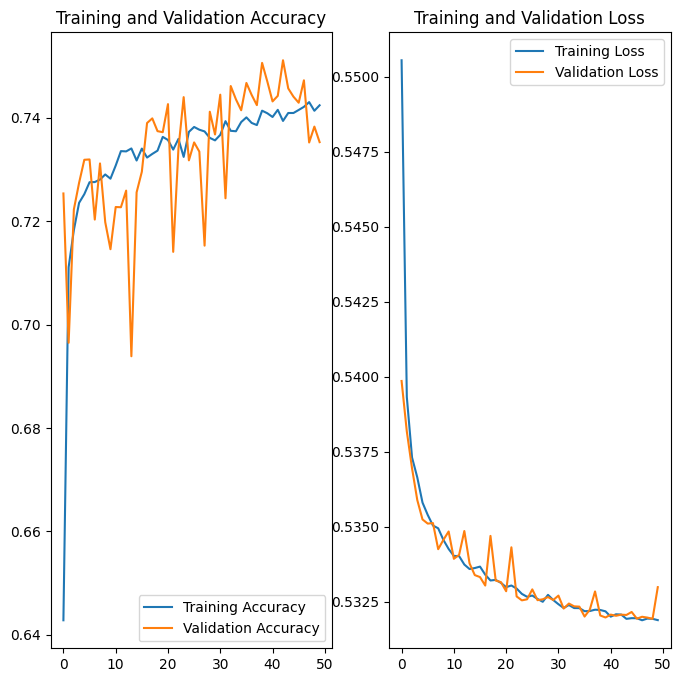
\includegraphics[width=0.75\textwidth]{autoencoder_train_1}
  \caption{First training of the autoencoder}
  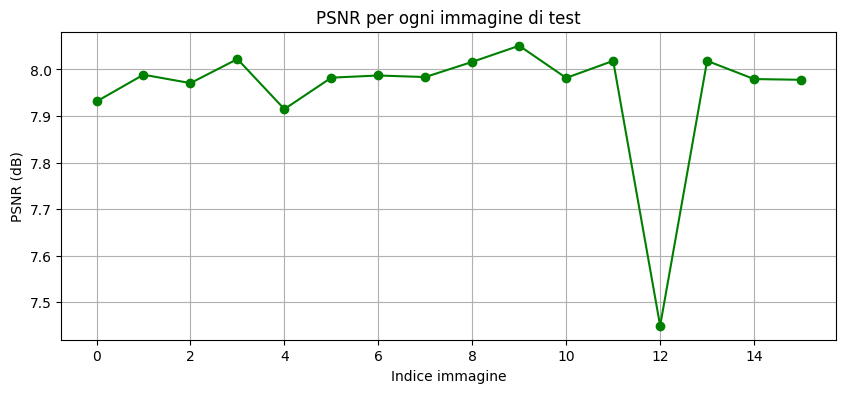
\includegraphics[width=0.75\textwidth]{autoencoder_psnr_1}
  \caption{First psnr of the autoencoder}
  \label{fig:auto_train_1}
\end{figure}

\subsection{RIDNet}
Model: "functional\_5"\\
\begin{tabular}{|| c | c | c | c ||}
  \hline
  Layer (type) & Output Shape & Param \# & Connected to \\
  \hline
  input\_layer\_5 & (None, None, None, 3) & 0 & - \\
  \hline
  mean\_shift\_10 & (None, None, None, 3) & 0 & input\_layer\_5[0][0] \\
  \hline
  conv2d\_250 (Conv2D) & (None, None, None, 32) & 896 & mean\_shift\_10[0][0] \\
  \hline
  block\_20 (Block) & (None, None, None, 32) & 93,666 & conv2d\_250[0][0] \\
  \hline
  block\_21 (Block) & (None, None, None, 32) & 93,666 & block\_20[0][0] \\
  \hline
  block\_22 (Block) & (None, None, None, 32) & 93,666 & block\_21[0][0] \\
  \hline
  block\_23 (Block) & (None, None, None, 32) & 93,666 & block\_22[0][0] \\
  \hline
  conv2d\_299 (Conv2D) & (None, None, None, 3) & 867 & block\_23[0][0] \\
  \hline
  mean\_shift\_11 & (None, None, None, 3) & 0 & conv2d\_299[0][0] \\
  \hline
  add\_413 (Add) & (None, None, None, 3) & 0 & mean\_shift\_11[0][0] \\
  \hline
\end{tabular}

 Total params: 376,427 (1.44 MB)\\
 Trainable params: 376,427 (1.44 MB)\\
 Non-trainable params: 0 (0.00 B)\\

 \begin{figure}
  \centering
  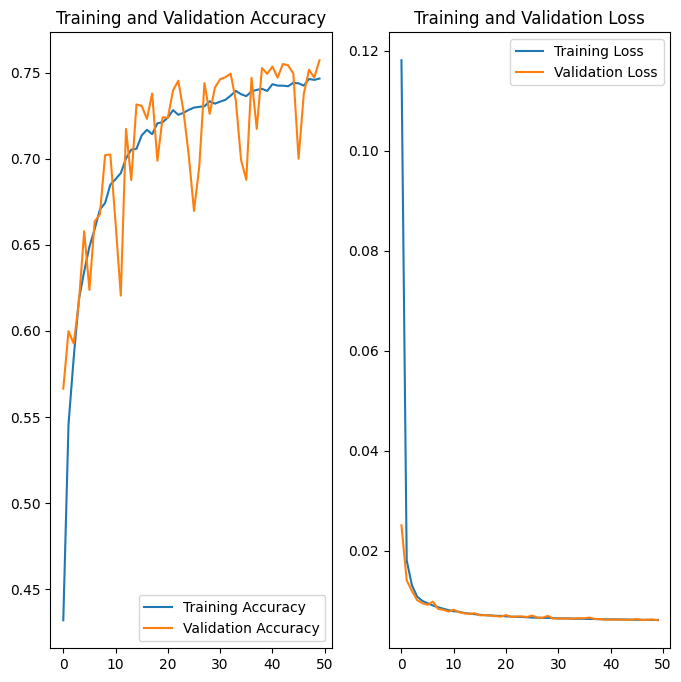
\includegraphics[width=0.75\textwidth]{ridnet_train_1}
  \caption{First training of the autoencoder}
  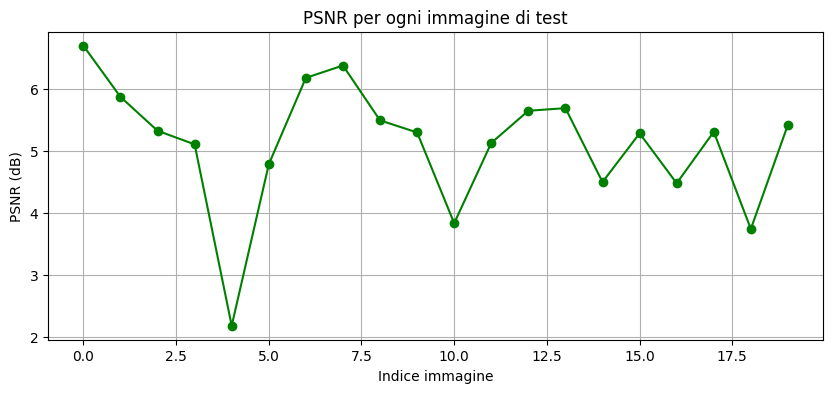
\includegraphics[width=0.75\textwidth]{ridnet_psnr_1}
  \caption{First psnr of the autoencoder}
  \label{fig:ridnet_train_1}
\end{figure}


 
\TODOComment{Aggiungere codice del pnrr}



\section{Quantizzazione dei modelli}
\section{Analisi dei modelli}
\subsection{Performance su dataset sconosciuti}



\chapter{Bibliografia}
\begin{itemize}
    \item \href{<sito>}{<nome>}
\end{itemize}
\end{document}




